%%%%%%%%%%%%%%%%
% switch from arc to beamer
%%%%%%%%%%%%%%%%
\PassOptionsToClass{a4paper,10pt}{article} % for article mode 
\PassOptionsToClass{aspectratio=1610,10pt}{beamer} % for beamer, handout, trans modes
\newcommand*{\BeamerswitchSpawn}[1]{ 
\ShellEscape{... -jobname=\jobname#1 \jobname} %
}
\documentclass{beamerswitch}
\mode<article>{
    \usepackage[top=3cm, bottom=3cm, left=3cm, right=3cm]{geometry}
}
\mode<presentation>{
    \usefonttheme[onlymath]{serif}
}

\usepackage{amsmath, amsthm, amsfonts}
\usepackage{subfiles, bm, hyperref, graphicx, listings}
\usepackage{authblk}
\usepackage{subcaption}

% my cmd
%%%%%%%%%%%%%%%%
% start my commands
%%%%%%%%%%%%%%%%
\newcommand{\lm}{\lambda_\textrm{max}}
\newcommand{\trace}{\mathbf{trace}}
\newcommand{\diag}{\mathbf{diag}}
\newcommand{\model}[1]{(\textbf{#1})}
\newcommand{\mx}{\mathbf{\max}\;}
\newcommand{\mn}{\mathbf{\min}\;}
\newcommand{\st}{\mathrm{s.t.\;}}
\newcommand{\ex}{\mathbb E}
\newcommand{\dx}{\;\bm dx}
\newcommand{\pr}{\mathbb P}
\newcommand{\id}{\mathbb I}
\newcommand{\bp}{\mathbb P}
\newcommand{\be}{\mathbb E}
\newcommand{\bi}{\mathbb I}
\newcommand{\bxi}{\bm \xi}
\newcommand{\bo}{\bm \omega}
\newcommand{\va}{\mathbf{Var}}
\newcommand{\dif}{\mathbf{d}}
\newcommand{\minp}[2]{\min\{#1, #2\}}
\newcommand{\intp}{\mathbf{int}}
\newcommand{\apex}{\mathbf{apex}}
\newcommand{\conv}{\mathbf{conv}}
%%%%%%%%%%%%%%%%
% finish my commands
%%%%%%%%%%%%%%%%

% theorem environments
\newtheorem{thm}{Theorem}[section]
\newtheorem{defn}[thm]{Definition}
\newtheorem{cor}[thm]{Corollary}
\newtheorem{lem}[thm]{Lemma}
\newtheorem{remark}[thm]{Remark}
% my code style
%%%%%%%%%%%%%%%%
% start my commands
%%%%%%%%%%%%%%%%
\lstdefinestyle{codestyle}{
    basicstyle=\ttfamily\footnotesize,
    tabsize=2
    \scriptsize
}
\title{Notes on Stochastic Programming}

\begin{document}

\author[1]{\small Chuwen Zhang}
\author[1]{\small Jingyuan Yang}
\affil[1]{\footnotesize Stochastic Programming Reading Group}

\maketitle
\section{Preface}

This monograph records the reading notes for the subject ``stochastic programming'' starting from Spring 2022. The goal is to increase the authors' familiarity in this fascinating field.
\section{Mathematical Background}
The part is based on \cite{shapiro_lectures_2014}, \cite{birge_introduction_2011} and so forth.
\subsection{Basic Convex Analysis}

Firstly, we introduce some definitions.
\begin{table}[h!]
    \centering
    \begin{tabular}{l|l}
        \(K_C\)          & recession cone  to set \(C\) \\
        \(C^0\)          & polar cone to set \(C\)      \\
        \(C^*\)          & dual cone to set \(C\)       \\
        \(\mathcal N_C\) & normal cone to set \(C\)     \\
        \(\mathcal R_C\) & radial cone to set \(C\)     \\
        \(\mathcal T_C\) & tangent cone to set \(C\)
    \end{tabular}
    \caption{A summary of convex sets}
\end{table}

The \autoref{fig:cone-illustration} give a clue to these special sets.
\begin{figure}[h!]
    \centering
    \begin{subfigure}[b]{0.3\textwidth}
        \centering
        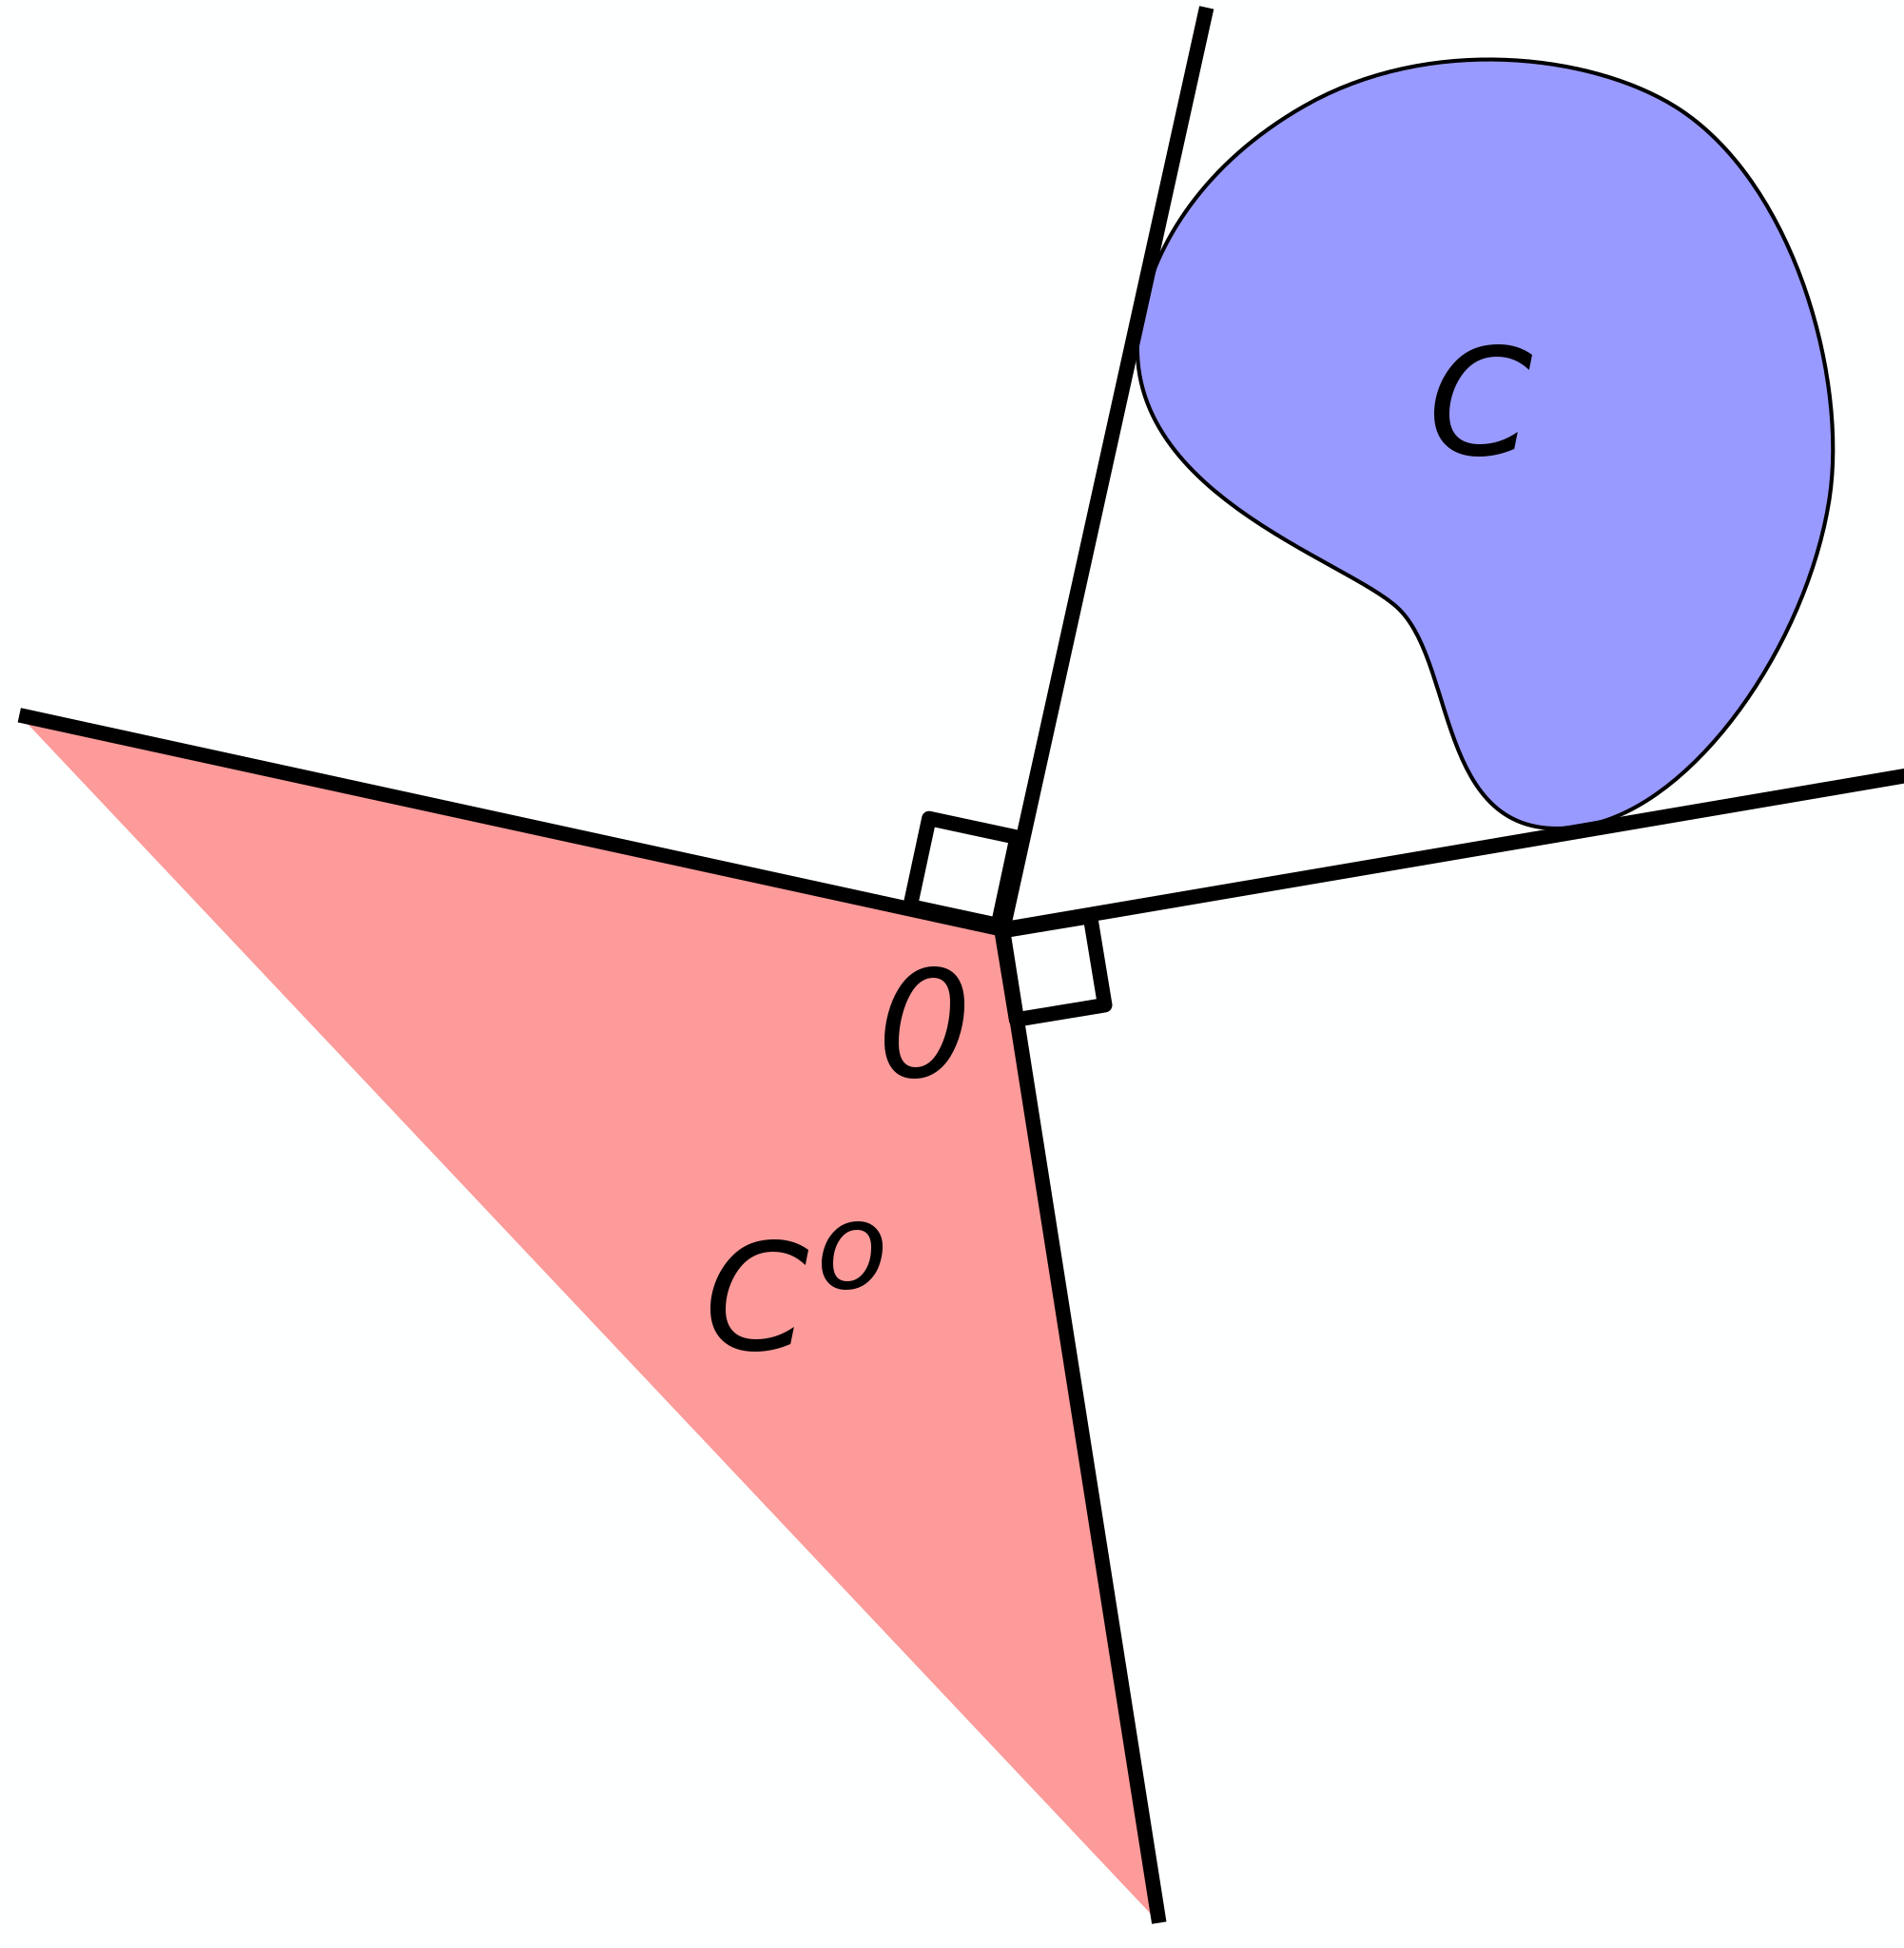
\includegraphics[width=1\linewidth]{figs/Polar_cone_illustration.png}
        \caption{The polar cone of \(C\)}
        \label{fig:polar-cone}
    \end{subfigure}
    \begin{subfigure}[b]{0.3\textwidth}
        \centering
        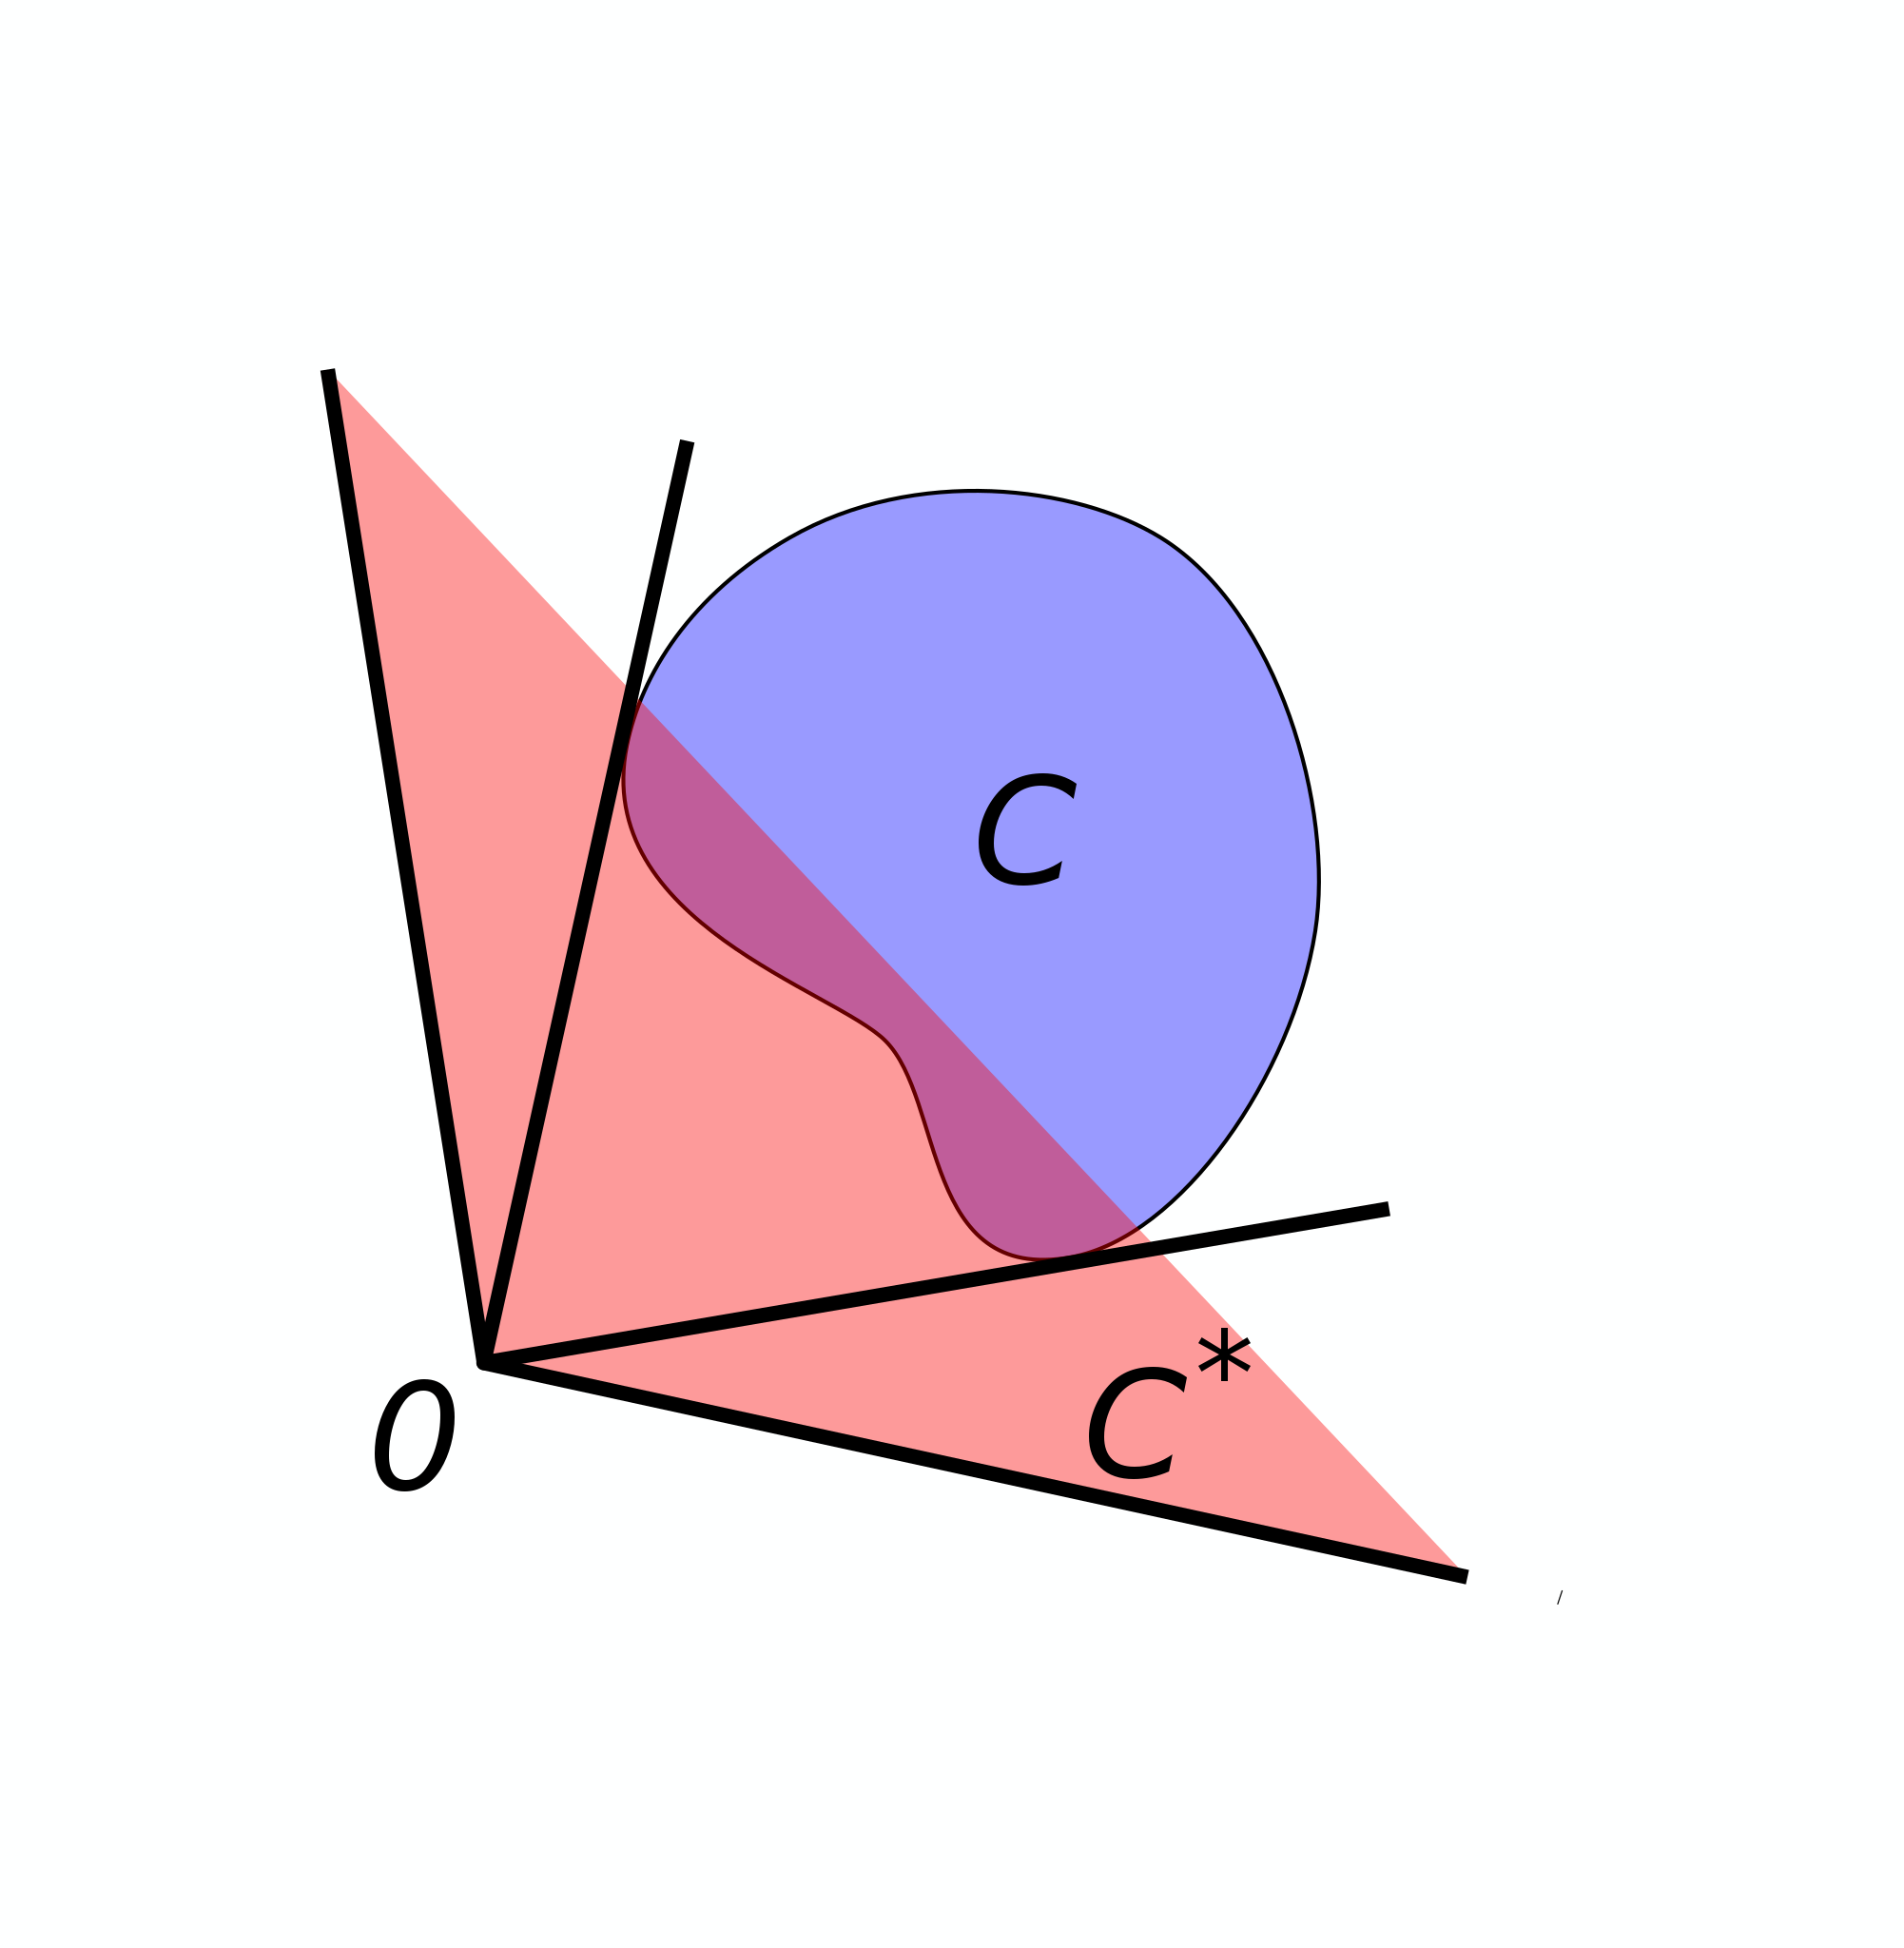
\includegraphics[width=1\linewidth]{figs/Dual_cone_illustration.png}
        \caption{The dual cone of \(C\)}
        \label{fig:dual-cone}
    \end{subfigure}
    \vskip\baselineskip
    \begin{subfigure}[b]{0.4\textwidth}
        \centering
        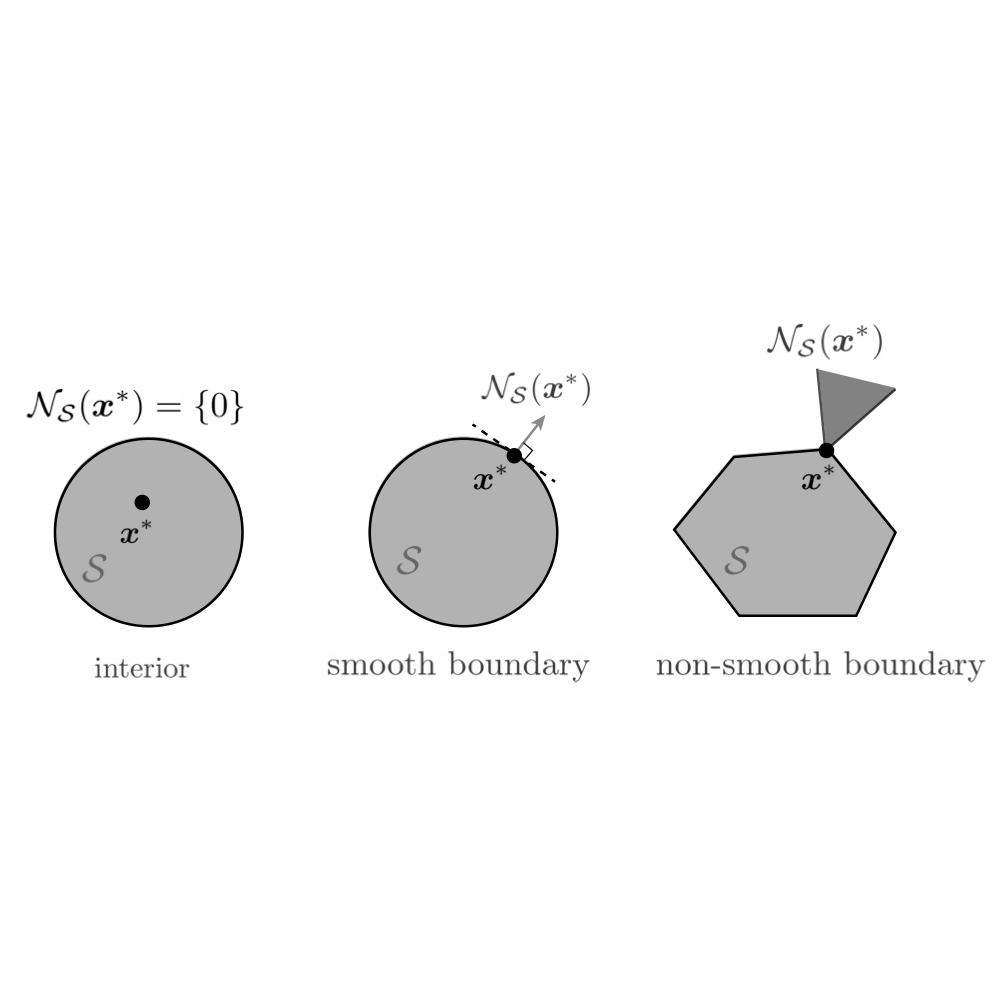
\includegraphics[width=1\linewidth]{figs/Normal_cone_illustration.svg.png}
        \caption{The normal cone of \(C\)}
        \label{fig:normal-cone}
    \end{subfigure}
    \begin{subfigure}[b]{0.3\textwidth}
        \centering
        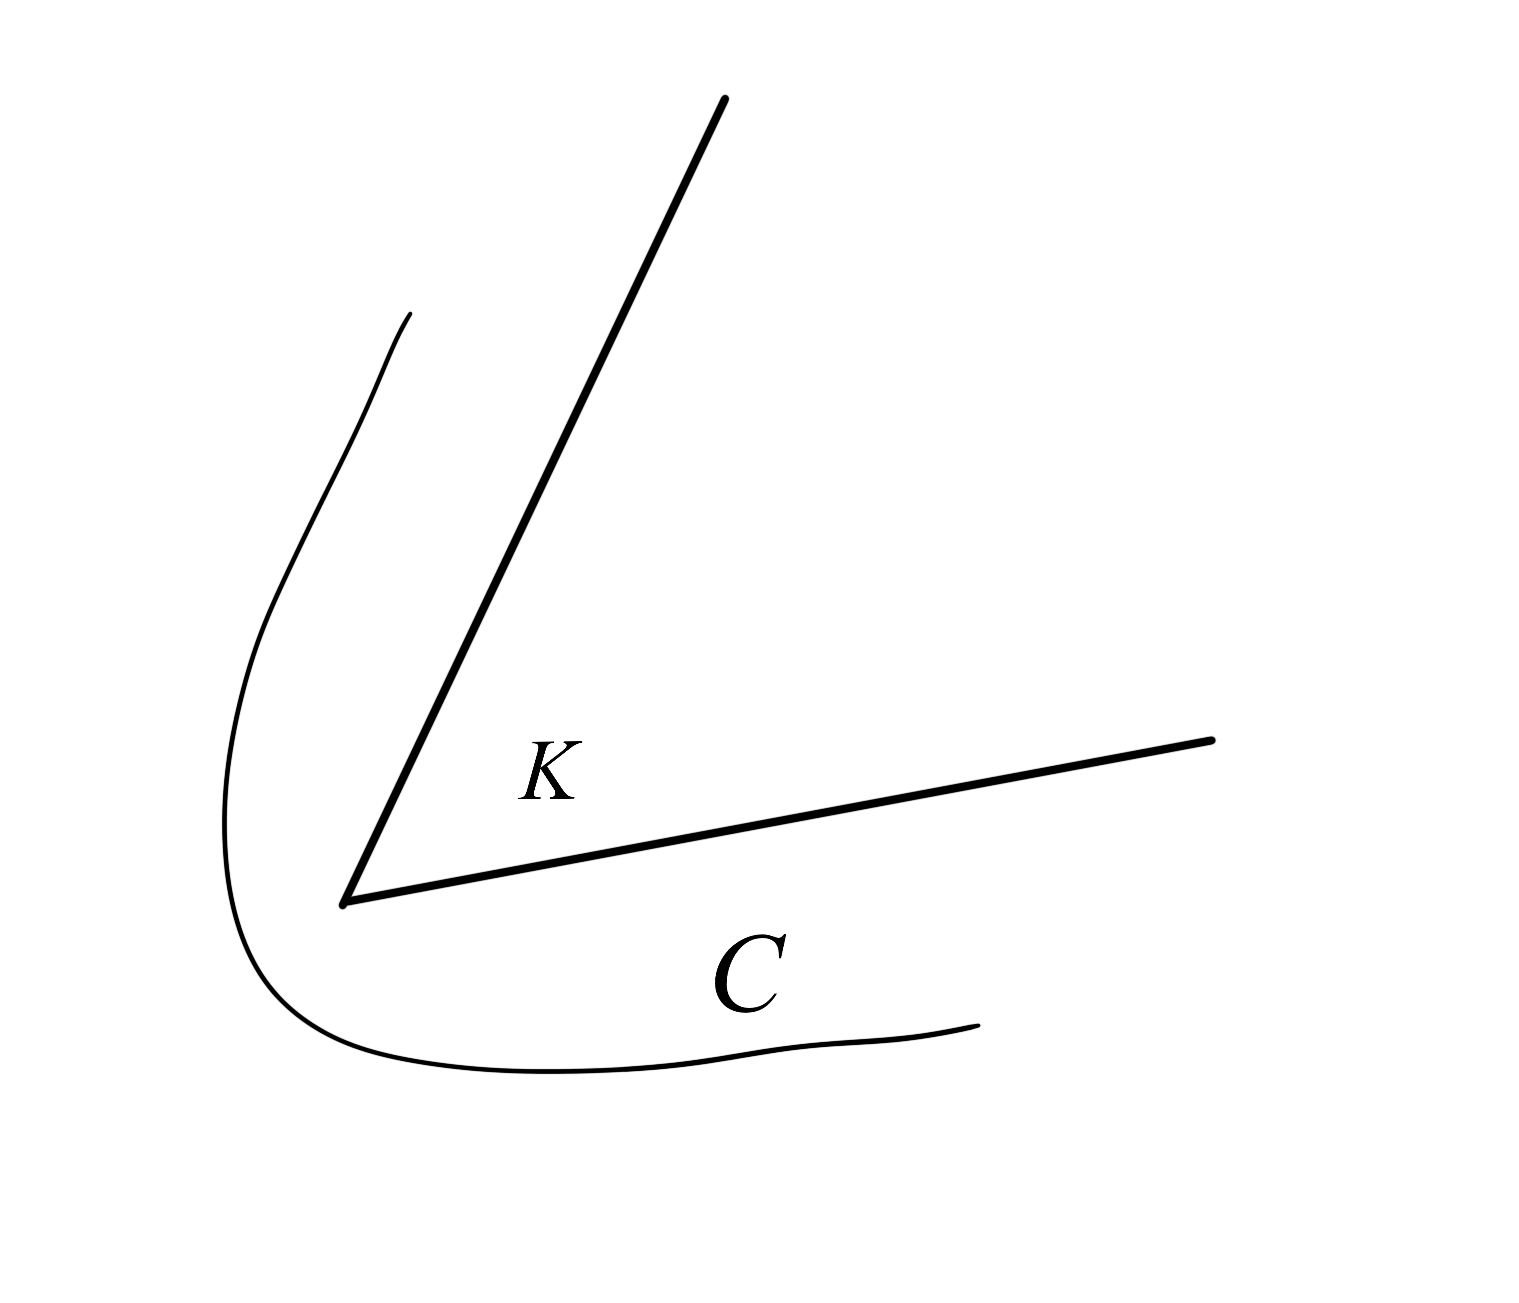
\includegraphics[width=1\linewidth]{figs/recession.png}
        \caption{The recession cone of \(C\)}
        \label{fig:recession-cone}
    \end{subfigure}
    \begin{subfigure}[b]{0.4\textwidth}
        \centering
        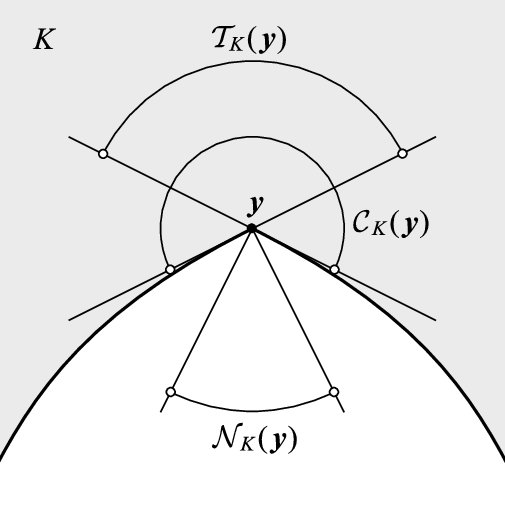
\includegraphics[width=1\linewidth]{figs/Contingent-tangent-and-normal-cone-on-a-non-convex-set-K-R-2_Q640.jpeg}
        \caption{Another example}
        \label{fig:another-cone}
    \end{subfigure}
    \caption{Illustration of the cones}
    \label{fig:cone-illustration}
\end{figure}

Understanding the definition of the cones is not an easy task, which requires materials in a set of books for convex analysis in different views.

\begin{defn}[The Minkowski Summation]
    If \(\emptyset \neq A, B \subset X\), the Minkowski sum of \(A\) and \(B\) is \(A+B:=\{ a+ b \mid a \in A, b \in B\}\). Moreover,
    \begin{enumerate}[(i)]
        \item if $x \in X, \lambda \in R$ and $\emptyset \neq \Gamma \subset R$, then $x+A:=A+x:=A+\{x\}, \Lambda \cdot A=\{\gamma a \mid \lambda \in \Lambda, a \in A\}$ and $\lambda A:=\{\lambda\} \cdot A$.
        \item We shall consider that $A+\emptyset=\emptyset$ and $\lambda \cdot \emptyset=\emptyset \cdot A=\emptyset$.
    \end{enumerate}
\end{defn}
\begin{defn}[The spaces in general vector spaces]
    In a vector space \(X\), the linear (subspace), affine space, cone, and convex set are,
    subspace of \(X\) that is closed under \((\cdot)\) combinations.
\end{defn}
\begin{defn}[The equivalent definitions of the \((\cdot)\) hulls]
    The two definitions are equivalent.
    \begin{enumerate}[(i)]
        \item The \((\cdot)\) hull of \(A \subset X\) is the \((\cdot)\) combinations of \(\{x\} \subseteq A\)
        \item The \((\cdot)\) hull of \(A\) can be represented as the following,
              \begin{equation}
                  (\cdot) (A) = \bigcap_V\{V \subset X \mid A \subseteq V, V (\cdot)\}
              \end{equation}
    \end{enumerate}
\end{defn}
% \begin{lem}[Minkowski sum and convex hull]
%     For all non-empty subsets \(S_1\) and \(S_2\) of a real vector space, the convex hull of their Minkowski sum is the Minkowski sum of their convex hulls:
%     \[\displaystyle \conv (S_{1}+S_{2})=\conv (S_{1})+\conv (S_{2}).\]
% \end{lem}
\begin{defn}[The basic convex sets]

    \begin{enumerate}[(i)]
        \item The recession cone \(K_C\) of the set \(C\) is formed by vectors \(h\) such that for any \(x \in C\) and any \(t > 0\) it follows that \(x + t\cdot h \in C\).
        \item The polar cone,
              \begin{equation}C^{0}=\left\{y:\langle y, x\rangle \leq 0 \quad \forall x \in C\right\}
              \end{equation}
              is the opposite of dual cone.
        \item The normal cone of \(C\) is,
              \begin{equation}
                  \mathcal N_C(x) = \{y: \langle y,  z-x \rangle \le 0, \forall x \in C\}
              \end{equation}
        \item The radial cone \(\mathcal R_C(x_0) = \bigcup_{t>0}\{ t(C - x_0) \}\).
        \item The tangent cone \(\mathcal T_C(x_0)\) is called the tangent cone to \(C\) at \(x_0\)
    \end{enumerate}

\end{defn}
\begin{thm}[The theorems for the recession cone]

    \begin{enumerate}[(i)]
        \item The \(K_C\) is convex if \(C\) is convex, and is closed if the set C is closed.
        \item The convex set C is bounded iff. \(K_C = \{0\}\)
        \item We have \(C = K_C + C\) by the Minkowski sum.
        \item If \(C\) is nonempty, closed, and convex, then
              \[K_C = \bigcap_{t> 0} t(C-a), \forall a \in C\]
    \end{enumerate}
\end{thm}

\begin{remark} The case where \(C\) is a polyhedron.
    Consider polyhedron \(C = \{x: Ax \le b\}\), based on definition,
    \begin{itemize}
        \item The recession cone is \(K_c = \{x: Ax \le 0\}\). Compare to the null space of \(A\), i.e., \(K_c \supseteq \mathbf{Null}(A)\)
    \end{itemize}
\end{remark}

\begin{thm}[Farkas Lemma]
    Consider \(Ax = b\), then either of the following in True:
    \begin{enumerate}[(i)]
        \item There exists \(x \ge 0\) such that \(Ax = b\)
        \item There exists \(y\) such that \(y^TA \ge 0, b^Ty < 0\)
    \end{enumerate}
\end{thm}

Farkas Lemma is very important in the Linear programming and convex optimization.
\begin{proof}
    (0) Method 0, Direct proof.
    (1) Method 1, using LP duality. But actually, LP duality is derived from Farkas Lemma.
    (2) Method 2, using Fourier–Motzkin elimination.
    (3) Method 3, use the separating hyperplane theorem of a convex set, see general Farkas Theorem
\end{proof}

\begin{thm}[General Farkas Theorem]
    Let $f, g_{1}, \ldots, g_{m}: R ^{n} \rightarrow R$ be convex functions, $C \subseteq R ^{n}$ a convex set, and let us assume that the Slater condition holds for $g_{1}, \ldots, g_{m}$; i.e., there exists an $\bar{x} \in \operatorname{rel} \operatorname{int} C$ such that $g_{j}(\bar{x})<0, j=1, \ldots$, m. The following two statements are equivalent:
    \begin{enumerate}[(i)]
        \item  The system below is not solvable,
              \begin{align*}
                  \begin{aligned}
                      f(x)     & <0                           \\
                      g_{j}(x) & \leq 0, \quad j=1, \ldots, m \\
                      x        & \in C
                  \end{aligned}
              \end{align*}
        \item  There are $y_{1}, \ldots, y_{m} \geq 0$ such that
              \begin{align*}
                  f(x)+\sum_{i=1}^{m} y_{j} g_{j}(x) \geq 0
              \end{align*}
              for all $x \in C$.
    \end{enumerate}
\end{thm}
\begin{proof}
    To prove this, one consider the set \(\{(u, \bm v): f(x) < u, \bm g(x) \le \bm v\}\), then show that \((0, \bm 0)\) does not in the set by the separating argument.
\end{proof}

\begin{remark}
    There are many ways to understand the Farkas lemma and the Farkas theorem. One way to see this is that the Farkas is to answer the question,

    \[g(x) \ge 0 \Rightarrow f(x) \ge 0?\]

    If true, can we do this by linear aggregation?
\end{remark}

\section{Two-Stage Problems}

\begin{frame}[allowframebreaks]{Introduction}
    To understand the difficulties of multistage (integer) programs, we first look at the structural properties of the value functions.

    Consider the two-stage problem,
    \begin{align*}
        \min_{x \in \mathcal X }~ & c^T x+ \mathcal Q (x)        \\
        \st                       & A x \leq b, x \in \mathcal X
    \end{align*}
    where the second stage recourse, the value function \(\mathcal Q (x) \) is defined as the expectation with a recourse variable \(y\).
    \begin{align*}
        \mathcal Q (x) & = \ex Q(x, \bxi)                                \\
                       & \bxi(\omega)    = (T, W, h )(\omega)            \\
                       & T(\bo) x+W(\bo) y=h(\bo), y \geq 0, \forall \bo \\
        Q(x, \bxi)     & = \min_{y \in \mathcal Y} q^T y
    \end{align*}

    \begin{remark}
        \begin{itemize}
            \item Assume random variable \(\bo \) living on some probability space, \((\Omega,\mathcal F, P)\)
            \item The first stage variable \(x\) is made before a realization of \(\bxi\), i.e., the ``here-and-now'' ones.
            \item The second stage variable \(y\), to be precise, should be \(\bm y(\omega)\) that actually depends on \(\bo\)
        \end{itemize}
    \end{remark}
\end{frame}
\begin{frame}[allowframebreaks]{Analysis on the value function}


    We first assume \((x, y)\) are continuous, for example, \(\mathcal X, \mathcal Y\) are convex. Define the function the support function \(s_{q}(\chi)\) of set \(\Pi(q)\), we notice,
    \begin{align*}
        \chi                    & = h - Tx                                                        \\
        \Pi(q)                  & \doteq \left\{\pi: W^{\top} \pi \leq q\right\}                  \\
        s_{q}(\chi)             & \doteq \inf \left\{q^{\top} y: W y=\chi, \quad y \geq 0\right\} \\
        \Rightarrow s_{q}(\chi) & =\sup _{\pi \in \Pi(q)} \pi^{\top} \chi
    \end{align*}

    Obviously,
    \begin{theorem} The value function \(Q(x, \bxi) = s_q(\chi)\), furthermore
        \begin{enumerate}
            \item Q is a homogeneous polyhedron function supporting \(\Pi(q)\)
            \item Also, the subdifferential of \(Q\) could also be defined.
                  \begin{align*}
                      \partial Q\left(x_{0}, \bxi\right)=-T^{\top} \mathcal D \left(x_{0}, \bxi\right)
                  \end{align*}
                  where
                  \begin{align*}
                      \mathcal  D (x, \bxi) = \pi ^* \doteq \arg \max _{\pi \in \Pi(q)} \pi^{\top}(h-T x)
                  \end{align*}
        \end{enumerate}
    \end{theorem}
    \section{Analysis on Value Function}
    Now we inspect the existence of \(Q\). Firstly, we introduce the definition,
    \begin{definition}
        Classification of recourse.
        The recourse problem is,
        \begin{enumerate}[i]
            \item (Fixed) if the matrix \(W(\bo) = W\) is fixed (not random).
            \item (Complete) if the system \(\{y: Wy = \chi, y \ge 0\}\) has a solution for every \(\chi\)
            \item (Simple) if both complete and fixed
            \item (Relatively complete) relatively complete if for every feasible \(x\),
                  the feasible set of the second-stage problem is nonempty for almost everywhere (a.e.) \(\bm \omega \in \Omega\).
        \end{enumerate}
    \end{definition}

    For a recourse to be complete, \(\Pi(q)\) must be bounded, i.e., the recession cone \(\Pi(0) = \{0\}\).

\end{frame}

\begin{frame}[allowframebreaks]
    \bibliography{robust}
    \bibliographystyle{apalike}
\end{frame}
\end{document}